% Chapter 'Evaluation'

\section{Methods}
	\subsection{Hypothesis}
		There are many things we could evaluate, as both features, segmentation, and classification are critical parts of the application. Even if only evaluating on the classifier, the number of combinations of features, and parameters of features (window size and window skip), is huge. We want keep a single independent variable. To limit ourselves, we chose not to test any combinations of features, but rather single features one at a time. We will then test that feature for $K \in [1;10]$. We state the null hypothesis that two knn-classifiers with a different k and otherwise identical, will not have result in significantly different confusion tables.
		
		This will be tested for each feature and each feature configuration.
		We will test window sizes of 20ms, 10ms, and 5ms; and we will test window skips of 10ms, 5ms, 2ms respectively. This will be the case for all features using window: MFCC, Spectral Flux, Spectral Centroid, Spectral Skew, and Spectral Rolloff. Only the first 20 MFCC coefficients will be used. RMS and ZCR are calculated over the entire sound.
		
		To determine if the independent variable $k$ has any has any significant effect on resulting confusion tables, the chi squared test is used. The probability calculated will be divided with the number of test to correct it over many tests, also called the Bonferroni correction\citep{bonferroni}.
		Since we are testing over 10 different K, the amount of tests done in total will be $Tests = 10*9/2$.
		We have chosen that the null hypothesis can be disputed, if any calculated $prob < alpha$, with $alpha=0.01$.
		
	\subsection{Measures}
		A confusion table is created for each test (each unique combination of variables). This will be shown in percentages (or rather, values between 0 and 1). Overall accuracy is calculated, along with precision, recall, and F-score for each class individually. For the sake of compactness, all the measures are included in an extended confusion table, as shown in the explanatory table \ref{table:eval:explanatory}. 
		The most important measure, for the sake of measuring our transcription system, would be the precision, that is, the amount of correctly transcribed sounds over the actual amount of that sound class.
		Recall should just be ignored, since we only test on the dataset, which means that we always test on all available samples of any given class, meaning that it would be the same as the amount of . This would be different, had the segmentation been part of the evaluation. It is included nonetheless, as further progress with this project might find a need for it.

			\begin{table}
				\centering
				\begin{tabular}{|c | c | c | c | c |}
					\hline
				 & Real Class(1) & Real Class(2) & Real Class(3) & Precision\\ \hline
					Label(1)  & ... & ... & ... & ...\\ \hline
					Label(2)  & ... & ... & ... & ...\\ \hline
					Label(3) & ... & ... & ... & ...\\ \hline
					F-Score & ... & ... & ... & Accuracy \\ \cline{1-4}
				\end{tabular}
				\caption{$K=1$}
				\label{table:eval:explanatory}
			\end{table}
		
		
	\subsection{Training and Test Sets}
		The dataset consists of sound segments, segmented based on the annotations. This means that our segmentation of sound (present in our application), will not be part of the evaluation.
		The training and test sets of sounds for the KNN classifier are randomly chosen from the same pool (the dataset). It is distributed between the training and test set in a 70\%/30\% ratio, accordingly, for each class. This means there will not be a fixed number of sounds for each class (neither total nor divided), but rather a fixed distribution between the number of training and test sounds for each class. We can do this instead of e.g. k-fold cross validation, due to scale of our collected dataset. The ratio was suggested by our supervisor\footnote{Bob L. Sturm}. The composition of the entire dataset has been summarized in table \ref{table:eval:datasetComposition}. 
		Furthermore, all sounds with a duration less than the windowsize used for feature calculation, are removed before testing. This is done before splitting the dataset, such as to make sure we do not distort the 70/30 distribution.

		\begin{table}
			\centering
			\begin{tabular}{|l|r|r|}
					\hline
					Value  &  Count  & Percent \\ \hline
			      noise    &  150    & 10.19\% \\ \hline
			          k    &  466    & 31.66\% \\ \hline
			  undefined    &  130    &  8.83\% \\ \hline
			          s    &  331    & 22.49\% \\ \hline
			         hh    &  395    & 26.83\% \\ \hline
			      TOTAL    &  1472	 & 100.00\% \\ \hline

			\end{tabular}
			\caption{Dataset composition}
			\label{table:eval:datasetComposition}
		\end{table}
		
		
	\subsection{Test Implementation}		% REFERENCES TO APPENDIX!
		To ease the testing of the transcription system, some additional scripts were created: \texttt{prettyPrintTables.m}, \texttt{testPlots.m}, \texttt{printDataStats.m}, and \texttt{DoEverything.m}.
		The \texttt{printPrettyTables.m} script simply runs a test and formats the results in tables usable for \LaTeX, while \texttt{testPlots.m} creates plots for precision, recall, and F over K, including the overall accuracy in all three plots, and saves them as PNG images\footnote{\url{using: https://github.com/ojwoodford/export\_fig}}. They will not be described further, as they have no real functional effect on the system -  they are just helping facilitating the tests. These scripts are quite simple and well-commented, and thus should require no more than than a simple mention, as they do not include features, not already explained in chapter \ref{chapter:OurApproach}.
			
 
\section{Results}
	
	For all results found, some interpretation of the data and statistics will be presented, although it will be kept short due to the breadth of configurations tested. Further discussion about the relevance of the data, possible mistakes that affected results, or similar, will be covered in chapter \ref{chapter:Discussion}. Only the relevant results will be shown and discussed, based on the accuracy, however the other measures will be considered as well. All data can be found in appendix \ref{app:res}. 

	\subsection{Root Mean Square}
		\begin{figure}
		
			\centering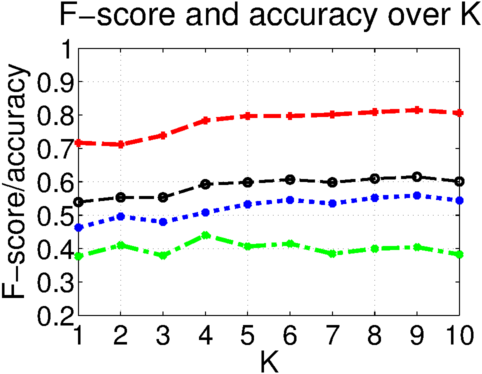
\includegraphics[width=0.3\textwidth]{tex/appendices/test/rms11FP.png}
			\centering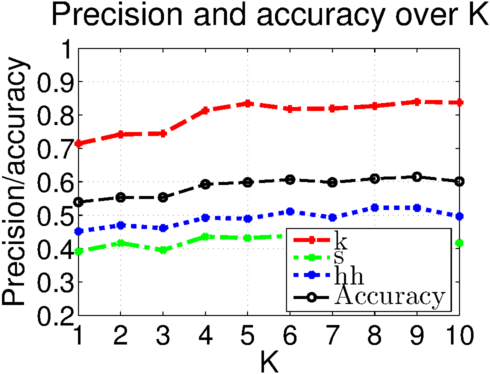
\includegraphics[width=0.3\textwidth]{tex/appendices/test/rms11_P.png}
			\centering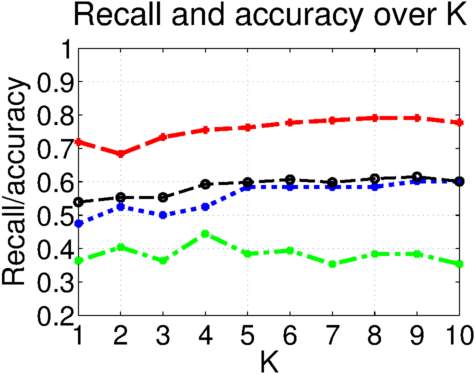
\includegraphics[width=0.3\textwidth]{tex/appendices/test/rms11_R.png}
			
			\label{fig:eval:rms}
			\caption{Plots over K for Root Mean Square}
		\end{figure}
	
		The best results using the RMS feature vector was observed using $K=9$, see table \ref{table:eval:rmsBest}. Some configurations had slightly higher precision in classes 's' and 'hh', although this seems minimal (see e.g. appendix  \ref{app:rms:k6) and \ref{app:rms:k8)}. The worst observed was using $K=1$, see table \ref{table:eval:rmsWorst}.
	
	
	
	\subsection{Zero Crossing Rate}
	
	\subsection{Mel Frequency Cepstrum Coefficients}
	
	\subsection{Spectral Centroid}
	
	\subsection{Spectral Skew}
	
	\subsection{Spectral Flux}

